The Groundwater Transport (GWT) Model \citep{modflow6gwt} in \mf represents the mass of solute in a cell as the sum of a dissolved part, held in the water in the cell, and a sorbed part, held on the solid aquifer material. Both parts are scaled by the water saturation, $S_w$, as shown by the storage terms on the left side of equation~\ref{eqn:gwtpde} of Chapter~\ref{ch:sorption},

\begin{equation}
\label{eqn:strandstorage}
\frac {\partial \left ( S_w \theta_m C \right )}{\partial t}
+ \hat{f}_m \rho_{b,m} \frac {\partial \left ( S_w \overline{C} \right ) }{\partial t} ,
\end{equation}

\noindent where $S_w$ is the water saturation ($L^3/L^3$), $\theta_m$ is the mobile-domain effective porosity ($L^3/L^3$), $C$ is the mobile-domain volumetric concentration of solute ($M/L^3$), $\hat{f}_m$ is the volume fraction of the mobile domain ($L^3/L^3$), $\rho_{b,m}$ is the bulk density of aquifer material in the mobile domain ($M/L^3$), and $\overline{C}$ is the concentration of sorbate ($M/M$).

Scaling the sorbed part by $S_w$ means that the mass of sorbate in a cell is proportional to the part of the cell that is saturated. When the water table falls and $S_w$ decreases, the sorbed mass in the cell decreases with it, and the mass that is given up is returned to the water that remains in the cell. Mass is conserved, but the solute that had been held on the solid aquifer material is redissolved into a shrinking volume of water and the simulated concentration rises. The solid aquifer material does not drain, however, and the sorbate that it carries does not move with the water table. The behavior is a consequence of the way the storage term is written, not a representation of a physical process.

The STRANDED\_MASS option of the Mobile Storage and Transfer (MST) Package holds the sorbed mass out of the mobile domain when a cell drains, and returns it when the cell rewets. The purpose of this chapter is to describe the formulation that was implemented, to show its effect for a cell with an oscillating water table, and to give an assessment of what the approach does and does not represent.

\subsection{Formulation}

A cell that uses the option carries an additional state variable, the stranded mass, which is a mass rather than a concentration. It is immobile: it is not advected, it takes no part in dispersion, and it is not transferred between cells. Writing it as a mass, and moving it into and out of the mobile domain in matched pairs, makes conservation a matter of bookkeeping rather than a property that has to be demonstrated.

\subsubsection{Drainage}

Over a time step in which the saturation of a cell decreases, the mass moved out of the mobile domain and into the stranded mass is

\begin{equation}
\label{eqn:strandrate}
\Delta M_{st} = \Delta S_w \, V_{cell} \, \hat{f}_m \rho_{b,m} \overline{C} ,
\end{equation}

\noindent where $\Delta M_{st}$ is the mass added to the stranded mass over the time step ($M$), $\Delta S_w$ is the decrease in saturation over the time step ($L^3/L^3$), and $V_{cell}$ is the volume of the cell ($L^3$). The right side of equation~\ref{eqn:strandrate} is the sorbed mass that the storage term would otherwise have released, so the two cancel and none of the sorbate that the cell gives up reaches the water that remains.

The sorbate concentration $\overline{C}$ depends on the unknown concentration through the sorption isotherm, so equation~\ref{eqn:strandrate} is added to the coefficient matrix and the right-hand side using the same linearization that the MST Package applies to the storage of sorbate for a nonlinear isotherm. For a linear isotherm the coefficient is $\Delta S_w V_{cell} \hat{f}_m \rho_{b,m} K_d / \Delta t$, where $K_d$ is the distribution coefficient ($L^3/M$) and $\Delta t$ is the length of the time step ($T$).

\subsubsection{Rewetting}

The stranded mass is taken to be distributed uniformly through the part of the cell that drained while the mass was held. A cell therefore carries, in addition to the stranded mass, the accumulated drained fraction $F$ that the stranded mass represents; $F$ increases by $\Delta S_w$ each time the cell drains and decreases by the increase in saturation each time the cell rewets. Over a time step in which the saturation increases by $\Delta S_w'$, the mass returned to the mobile domain is

\begin{equation}
\label{eqn:strandreturn}
\Delta M_r = M_{st} \, \min \left ( \frac{\Delta S_w'}{F}, 1 \right ) ,
\end{equation}

\noindent where $\Delta M_r$ is the mass returned over the time step ($M$) and $M_{st}$ is the stranded mass held by the cell at the start of the time step ($M$). Because $M_{st}$ is known from the previous time step, equation~\ref{eqn:strandreturn} is an explicit source of mass to the cell.

Measuring the returned share against $F$, rather than against the unsaturated part of the cell, makes returning the exact inverse of stranding. A cell that drains and then rewets by the same amount recovers all of the mass it gave up, and a cell that rewets part of the way recovers the corresponding share, because the mass in the part that remains drained stays there. The mass that returns is the mass that the same cell gave up; no neighboring cell is used, and no mass is created or discarded.

\subsubsection{Decay}

Stranded mass decays at the first-order rate specified for the sorbed phase, $\lambda_2$. The mass lost over a time step is

\begin{equation}
\label{eqn:stranddecay}
\Delta M_d = M_{st} \left ( 1 - e^{-\lambda_2 \Delta t} \right ) ,
\end{equation}

\noindent where $\Delta M_d$ is the mass lost to decay over the time step ($M$). A negative rate is production, following the convention used for the decay rates of the mobile domain, and because production is proportional to the mass held, a cell that holds no stranded mass produces none. Zero-order decay is not applied to the stranded mass, because a zero-order rate would drive an empty reservoir negative; a warning is issued if zero-order decay is active.

\subsubsection{Budget}

Three quantities change the stranded mass of a cell, and only one of them is decay,

\begin{equation}
\label{eqn:strandbalance}
\frac{d M_{st}}{d t} = \frac{\Delta M_{st}}{\Delta t} - \frac{\Delta M_r}{\Delta t} - \frac{\Delta M_d}{\Delta t} .
\end{equation}

The first two terms are transfers, exactly paired with the mobile domain, and are reported together as a single entry, STORAGE-STRANDED, in the model budget. Decay of stranded mass is different: it is mass that leaves the simulation without passing through the concentration equation. Reporting it in the model budget would leave that budget with an outflow that has no matching inflow and would drive the percent discrepancy away from zero. It is reported instead in a budget for the package, in the same way that the Immobile Storage and Transfer (IST) Package reports the budget of an immobile domain, together with the storage of the stranded mass and the transfer with the mobile domain. The mobile domain never sees the decayed mass; decay reduces the stranded mass, which reduces the mass available to return later.

The stranded mass of a cell is updated from the same quantities that are reported to the budget, once per time step rather than within the iteration of the nonlinear solution. Deriving the state and the reported rate from one number, rather than computing each separately, is what keeps the two from drifting apart.

\subsubsection{Definition of the change in saturation}

The change in saturation used in equations~\ref{eqn:strandrate} and~\ref{eqn:strandreturn} is the change that the storage terms of the MST Package use, which is obtained from the water released to or taken into storage by the flow model rather than from the geometry of the cell. Using the same quantity is what makes the mass held back cancel the mass that the storage term would otherwise have released, and is the reason the percent discrepancy of the model budget is unaffected by the option.

Solute held by water that does not drain, the residual water content of the unsaturated zone, is not represented. That process has no counterpart in the storage terms of the MST Package to cancel, and so would require a change in saturation defined from the geometry of the cell. Only the sorbed phase is stranded.

\subsection{Extension to Immobile Domains}

An immobile domain represented with the IST Package scales its mass by the water saturation in the same way that the mobile domain does, so an immobile domain also returns its solute to the water that remains when a cell drains. Stranding is a property of a domain rather than of a cell: a simulation with $nim$ immobile domains would require $nim + 1$ sets of stranded mass, one for the mobile domain and one for each immobile domain, because each domain carries its own bulk density, sorption parameters, and decay rates.

The formulation in this chapter is written in terms of the properties of a single domain, and the stranded mass is implemented as a separate module that the owning package supplies its properties to, with its own memory path, so that the IST Package can own a set of stranded mass without collision. Stranding the mass of an immobile domain would then use equations~\ref{eqn:strandrate} through~\ref{eqn:stranddecay} with the parameters of that domain and would report its transfer with the mobile domain in the budget of the IST Package.

Immobile domains are not supported in the present implementation. Specifying STRANDED\_MASS together with an active IST Package is an error rather than a warning, because a simulation in which the mobile domain holds its sorbate back while the immobile domains continue to release theirs is harder to interpret than one in which neither does. The transfer of mass between the mobile and immobile domains needs no change, because it is already scaled by the saturation and goes to zero as a cell dries.

\subsection{Example: Oscillating Water Table}

The effect of the option is shown for a single cell whose water table rises and falls. The cell is 100 by 100 meters in plan, extends from an elevation of 40 meters to an elevation of 0 meters, and has a mobile-domain porosity of 0.3 and a specific yield of 0.3. A constant head in the cell next to it varies sinusoidally with a period of 100 days about a mean of 24 meters with an amplitude of 14 meters, so that the saturation of the cell varies between about 0.25 and 0.95 over four cycles (fig.~\ref{fig:strandedmass}\textit{A}). The initial concentration is 100 grams per cubic meter throughout, and water entering through the constant head has a concentration of zero. Sorption is represented with a linear isotherm using a bulk density of 1,600 kilograms per cubic meter and a distribution coefficient of $1 \times 10^{-4}$ cubic meters per kilogram; where decay is active, the first-order rate is 0.005 per day for both the dissolved and the sorbed phase.

Five transport simulations were run on the same flow field. Simulated concentrations (fig.~\ref{fig:strandedmass}\textit{B}) rise as the cell drains in every case, because the water that remains occupies a smaller volume. Without sorption the peak concentration reaches 376 grams per cubic meter. Adding sorption lowers the peak to 313 grams per cubic meter, because sorbate buffers the dissolved concentration. Activating the stranded mass option lowers the peak further, to 261 grams per cubic meter, a reduction of 17 percent, because the sorbate that the cell gives up as it drains is held out of the mobile domain instead of being redissolved. With first-order decay active the peak concentration falls from 193 to 167 grams per cubic meter, a reduction of 13 percent.

The mass held out of the mobile domain (fig.~\ref{fig:strandedmass}\textit{C}) rises and falls with the water table, reaching about 2,400 kilograms at the driest part of each cycle and returning nearly to zero when the cell refills. With decay active the stranded mass is smaller, both because the concentration in the cell is lower and because the stranded mass decays while it is held, and the peak decreases over successive cycles. The percent discrepancy of the model budget remained at 0.00 for every time step of all five simulations.

\begin{figure}[!ht]
	\begin{center}
	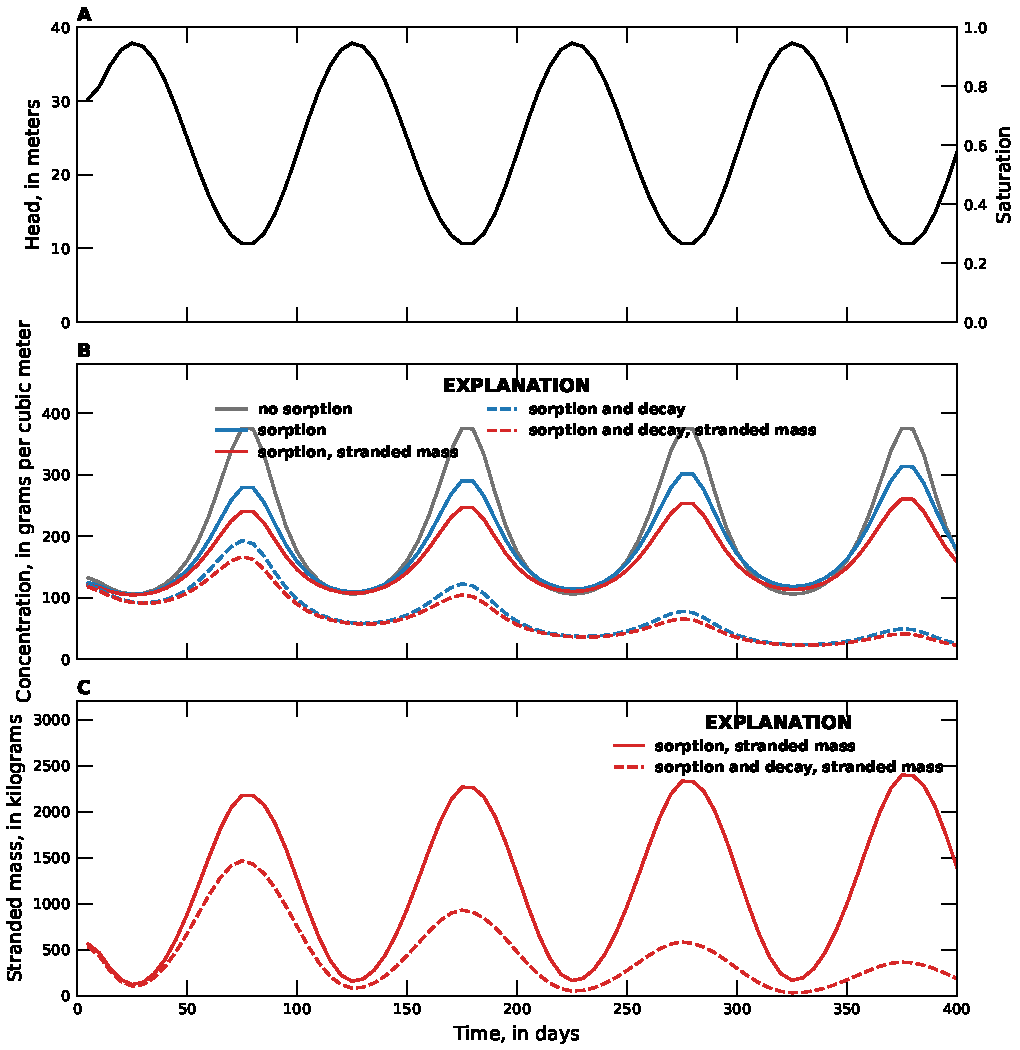
\includegraphics{./Figures/MSTStrandedMass.pdf}
	\caption[Graphs showing the effect of the stranded mass option for a cell with an oscillating water table]{Graphs showing the effect of the stranded mass option of the MST Package for a cell with an oscillating water table. The cell extends from an elevation of 40 meters to an elevation of 0 meters and has a mobile-domain porosity of 0.3, a specific yield of 0.3, a bulk density of 1,600 kilograms per cubic meter, a distribution coefficient of $1 \times 10^{-4}$ cubic meters per kilogram, and an initial concentration of 100 grams per cubic meter. \textit{A}, Simulated head in the cell and the corresponding water saturation; \textit{B}, simulated concentration for five combinations of sorption, first-order decay, and the stranded mass option; \textit{C}, mass held out of the mobile domain for the two simulations that use the stranded mass option}
	\label{fig:strandedmass}
	\end{center}
\end{figure}

\subsection{Assessment}

The approach is conservative by construction. The mobile domain loses exactly the mass that the stranded mass gains and gains exactly the mass that it loses, so the sum of the mobile and stranded mass changes only through decay and the flows across the boundaries of the model. There is no interpolation, no limiting, and no path that creates or discards mass, so a discrepancy in the model budget would indicate an error in the implementation rather than a modeling choice. This is a stronger property than that of the approaches available in MT3D-USGS \citep{mt3dusgs}, where a cell that rewets is assigned either an inverse-distance-weighted average of the concentrations of its neighbors, which creates mass, or a concentration of zero, which destroys it.

The approach is also an approximation, and it is worth being clear about what it does not represent.

\begin{itemize}

\item \textbf{The unsaturated zone is not simulated.} The stranded mass is held in place and returned when the cell rewets. It does not move, so solute cannot be carried downward through the unsaturated zone by infiltrating water, and it cannot be redistributed within the drained part of a cell. A simulation that needs those processes should represent the unsaturated zone explicitly with the Unsaturated Zone Flow (UZF) Package and the Unsaturated Zone Transport (UZT) Package, which is a considerably larger modeling commitment.

\item \textbf{Sorbate is held out of equilibrium.} Sorbate in the drained part of a cell is assumed to keep the mass it had when the cell drained. In reality the solid aquifer material above the water table remains in contact with the residual water, and the sorbed and dissolved phases of that water continue to interact. Assuming that the mass is held unchanged is defensible when the residual water is nearly immobile and the contact with the mobile domain is slight, and becomes less so as the drained interval becomes wetter.

\item \textbf{Solute in residual water is not represented.} Only the sorbed phase is stranded. Solute held by the water that does not drain is returned to the mobile domain as it is without the option, so the option does not remove the effect of drainage on the simulated concentration; it removes the part of that effect that comes from the solid phase. For a strongly sorbing solute that part is the larger one, and for a solute that does not sorb the option has no effect at all.

\item \textbf{The distribution within the drained interval is uniform.} The share of the stranded mass that returns is proportional to the share of the drained interval that rewets. A water table that falls slowly and rises quickly, or a cell that is thick relative to the range of the water table, will return mass in a different order than a model that resolved the vertical distribution would.

\end{itemize}

The option is intended for simulations in which the water table moves through cells that carry a substantial sorbed load and in which redissolving that load on drainage is a recognized artifact, and where representing the unsaturated zone explicitly is not warranted. Under those conditions it removes an artifact of the storage formulation without introducing a term that has to be calibrated: the mass that is held back is determined by the sorption parameters that the simulation already uses, and the option has no effect when sorption is not active.
